\chapter{Dimension Reduction Strategies}\label{Chap:DimRed}

In this section dimension reduction strategies are introduced. All dimension reduction strategies are based on the idea of finding the important directions in the original input space
in order to approximate the response on a lower dimensional space. Once a lower dimensional space is identified, several UQ strategies can be deployed on it making the UQ studies less computational expensive.

In the following two approaches are introduced, namely the Active Subspace method \cite{constantine2015active} and the Basis Adaptation \cite{Tip14}.

\section{Active Subspace Models}\label{Chap:ActSub}
The idea behind active subspaces is to find directions in the input variable
space in which the quantity of interest is nearly constant. After rotation of
the input variables, this method can allow significant dimension reduction. Below is a brief summary of the process.
\begin{enumerate}
\item Compute the gradient of the quantity of interest, $q = f(\mathbf{x})$,
    at several locations sampled from the full input space,
    $$\nabla_{\mathbf{x}} f_i = \nabla f(\mathbf{x}_i).$$

\item Compute the eigendecomposition of the matrix $\hat{\mathbf{C}}$,
    $$\hat{\mathbf{C}} = \frac{1}{M}\sum_{i=1}^{M}\nabla_{\mathbf{x}} f_i\nabla_{\mathbf{x}} f_i^T = \hat{\mathbf{W}}\hat{\mathbf{\Lambda}}\hat{\mathbf{W}}^T,$$
    where $\hat{\mathbf{W}}$ has eigenvectors as columns, 
    $\hat{\mathbf{\Lambda}} = \text{diag}(\hat{\lambda}_1,\:\ldots\:,\hat{\lambda}_N)$
    contains eigenvalues, and $N$ is the total number of parameters.

\item Using a truncation method or specifying a
    dimension to estimate the active subspace size, 
    split the eigenvectors into active and inactive directions,
    $$\hat{\mathbf{W}} = \left[\hat{\mathbf{W}}_1\quad\hat{\mathbf{W}}_2\right].$$
    These eigenvectors are used to rotate the input variables.

\item Next the input variables, $\mathbf{x}$, are expanded in terms of active and
    inactive variables,
    $$\mathbf{x} = \hat{\mathbf{W}}_1\mathbf{y} + \hat{\mathbf{W}}_2\mathbf{z}.$$

\item A surrogate is then built as a function of the active variables,
    $$g(\mathbf{y}) \approx f(\mathbf{x})$$
\end{enumerate}

As a concrete example, consider the function:~\cite{constantine2015active}
$$f(x) = \exp\left(0.7x_1 + 0.3x_2\right).$$
Figure \ref{fig:activesubspace}(a) is a contour plot of $f(x)$. The black arrows indicate the
eigenvectors of the matrix $\hat{\mathbf{C}}$. Figure \ref{fig:activesubspace}(b) is the same 
function but rotated so that the axes are aligned with the eigenvectors. We arbitrarily
give these rotated axes the labels $y_1$ and $y_2$. From fig.~\ref{fig:activesubspace}(b) it is
clear that all of the variation is along $y_1$ and the dimension of the rotated
input space can be reduced to 1.

\begin{figure}[htbp]
  \begin{subfigmatrix}{2}
  \subfigure[Original function]{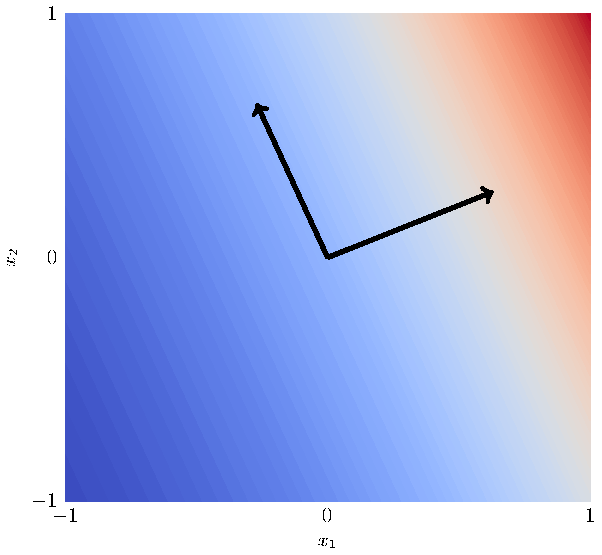
\includegraphics{images/unrotated_example}}
  \subfigure[Rotated function]{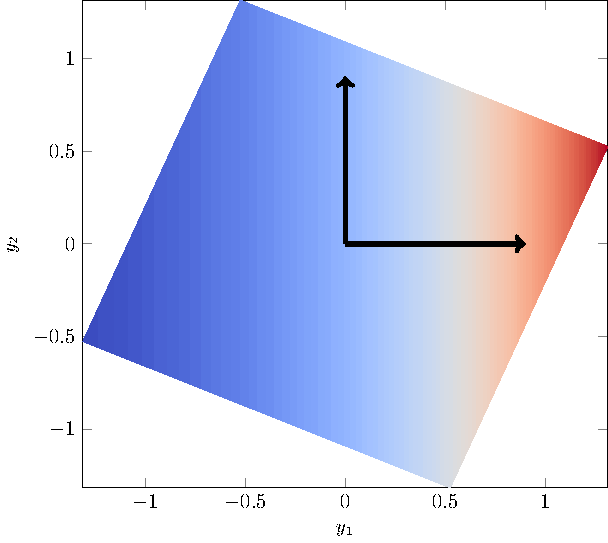
\includegraphics{images/rotated_example}}
  \end{subfigmatrix}
  \caption{Example of a 2D function with a 1D active subspace.}
\label{fig:activesubspace}
\end{figure}

For additional information, see references~\cite{Constantine-preprint-active,constantine2014active,constantine2015active}.

\subsection{Truncation Methods}\label{Sec:trunc}
Once the eigenvectors of $\hat{\mathbf{C}}$ are obtained we must decide how many
directions to keep. If the exact subspace size is known \textit{a priori} it can be
specified. Otherwise there are three automatic active subspace detection and
truncation methods implemented:
\begin{itemize}
\item Constantine metric (default),
\item Bing Li metric,
\item and Energy metric.
\end{itemize}

\subsubsection{Constantine metric}\label{SubSec:constantine}
The Constantine metric uses a criterion based on the variability of the subspace estimate. 
Eigenvectors are computed for bootstrap samples of the gradient matrix. The 
subspace size associated with the minimum distance between bootstrap 
eigenvectors and the nominal eigenvectors is the estimated active subspace
size.

Below is a brief outline of the Constantine method of active subspace 
identification. The first two steps are common to all active subspace 
truncation methods.
\begin{enumerate}
\item Compute the gradient of the quantity of interest, $q = f(\mathbf{x})$,
    at several locations sampled from the input space,
    $$\nabla_{\mathbf{x}} f_i = \nabla f(\mathbf{x}_i).$$

\item Compute the eigendecomposition of the matrix $\hat{\mathbf{C}}$,
    $$\hat{\mathbf{C}} = \frac{1}{M}\sum_{i=1}^{M}\nabla_{\mathbf{x}} f_i\nabla_{\mathbf{x}} f_i^T = \hat{\mathbf{W}}\hat{\mathbf{\Lambda}}\hat{\mathbf{W}}^T,$$
    where $\hat{\mathbf{W}}$ has eigenvectors as columns, 
    $\hat{\mathbf{\Lambda}} = \text{diag}(\hat{\lambda}_1,\:\ldots\:,\hat{\lambda}_N)$
    contains eigenvalues, and $N$ is the total number of parameters.

\item Use bootstrap sampling of the gradients found in step 1 to compute replicate
    eigendecompositions,
    $$\hat{\mathbf{C}}_j^* = \hat{\mathbf{W}}_j^*\hat{\mathbf{\Lambda}}_j^*\left(\hat{\mathbf{W}}_j^*\right)^T.$$

\item Compute the average distance between nominal and bootstrap subspaces,
    $$e^*_n = \frac{1}{M_{boot}}\sum_j^{M_{boot}} \text{dist}(\text{ran}(\hat{\mathbf{W}}_n), \text{ran}(\hat{\mathbf{W}}_{j,n}^*)) = \frac{1}{M_{boot}}\sum_j^{M_{boot}} \left\| \hat{\mathbf{W}}_n\hat{\mathbf{W}}_n^T - \hat{\mathbf{W}}_{j,n}^*\left(\hat{\mathbf{W}}_{j,n}^*\right)^T\right\|,$$
    where $M_{boot}$ is the number of bootstrap samples, 
    $\hat{\mathbf{W}}_n$ and $\hat{\mathbf{W}}_{j,n}^*$ both contain 
    only the first $n$ eigenvectors, and $n < N$.

\item The estimated subspace rank, $r$, is then,
    $$r = \operatorname*{arg\,min}_n \, e^*_n.$$
\end{enumerate}

For additional information, see Ref.~\cite{constantine2015active}.

\subsubsection{Bing Li metric}\label{SubSec:bingli}
The Bing Li metric uses a trade-off criterion to determine where to truncate the active subspace.
The criterion is a function of the eigenvalues
and eigenvectors of the active subspace gradient matrix. This function compares 
the decrease in eigenvalue amplitude with the increase in eigenvector variability
under bootstrap sampling of the gradient matrix. The active subspace size is taken to 
be the index of the first minimum of this quantity.

Below is a brief outline of the Bing Li method of active subspace 
identification. The first two steps are common to all active subspace 
truncation methods.
\begin{enumerate}
\item Compute the gradient of the quantity of interest, $q = f(\mathbf{x})$,
    at several locations sampled from the input space,
    $$\nabla_{\mathbf{x}} f_i = \nabla f(\mathbf{x}_i).$$

\item Compute the eigendecomposition of the matrix $\hat{\mathbf{C}}$,
    $$\hat{\mathbf{C}} = \frac{1}{M}\sum_{i=1}^{M}\nabla_{\mathbf{x}} f_i\nabla_{\mathbf{x}} f_i^T = \hat{\mathbf{W}}\hat{\mathbf{\Lambda}}\hat{\mathbf{W}}^T,$$
    where $\hat{\mathbf{W}}$ has eigenvectors as columns, 
    $\hat{\mathbf{\Lambda}} = \text{diag}(\hat{\lambda}_1,\:\ldots\:,\hat{\lambda}_N)$
    contains eigenvalues, and $N$ is the total number of parameters.

\item Normalize the eigenvalues,
    $$\lambda_i = \frac{\hat{\lambda}_i}{\sum_j^N \hat{\lambda}_j}.$$

\item Use bootstrap sampling of the gradients found in step 1 to compute replicate
    eigendecompositions,
    $$\hat{\mathbf{C}}_j^* = \hat{\mathbf{W}}_j^*\hat{\mathbf{\Lambda}}_j^*\left(\hat{\mathbf{W}}_j^*\right)^T.$$

\item Compute variability of eigenvectors,
    $$f_i^0 = \frac{1}{M_{boot}}\sum_j^{M_{boot}}\left\lbrace 1 - \left\vert\text{det}\left(\hat{\mathbf{W}}_i^T\hat{\mathbf{W}}_{j,i}^*\right)\right\vert\right\rbrace ,$$
    where $\hat{\mathbf{W}}_i$ and $\hat{\mathbf{W}}_{j,i}^*$ both 
    contain only the first $i$ eigenvectors and $M_{boot}$ is the 
    number of bootstrap samples. The value of the variability at the first index,
    $f_1^0$, is defined as zero.

\item Normalize the eigenvector variability,
    $$f_i = \frac{f_i^0}{\sum_j^N f_j^0}.$$

\item The criterion, $g_i$, is defined as,
    $$g_i = \lambda_i + f_i.$$

\item The index of first minimum of $g_i$ is then the estimated active 
    subspace rank.
\end{enumerate}

For additional information, see Ref.~\cite{bing-li}.

\subsubsection{Energy metric}\label{SubSec:energy}
The energy metric truncation method uses a criterion based on the derivative matrix
eigenvalue energy. The user can specify the maximum percentage (as a decimal) of
the eigenvalue energy that is not captured by the active subspace represenation.

Using the eigenvalue energy truncation metric, the subspace size is determined using the following equation:
$$n = \inf \left\lbrace d \in \mathbb{Z} \quad\middle|\quad 1 \le d \le N \quad \wedge\quad 1 - \frac{\sum_{i = 1}^{d} \lambda_i}{\sum_{i = 1}^{N} \lambda_i} \,<\, \epsilon \right\rbrace $$
where $\epsilon$ is the \texttt{truncation\_tolerance}, $n$ is the estimated subspace size, $N$ is the size of the full space, and $\lambda_i$ are the eigenvalues of the derivative matrix.

%%%%%%%%%%%%%%%%%%%%%%%%%%%%%%%%%%%%%%%%%%%%%%%%%%%%%%%%%%%%%%%%%%%%%%%%%%%%%%%%%%%%%%%%%%%%%%%%%%

%%%%%%%%%%%%%%%%%%%%%%%%%%    BASIS ADAPTATION

%%%%%%%%%%%%%%%%%%%%%%%%%%%%%%%%%%%%%%%%%%%%%%%%%%%%%%%%%%%%%%%%%%%%%%%%%%%%%%%%%%%%%%%%%%%%%%%%%%
\section{Basis Adaptation Models}\label{Chap:BasAdapt}
The idea behind the basis adaptation is similar to the one employed in the active subspaces that is to find the directions
in the input space where the variations of the QoI are negligible or they can be safely discarded, \textit{i.e.} without significantly affecting the QoI's statistics, 
according to a truncation criterion. One of the main differences between the basis adaptation and
the active subspaces strategy is that the basis adaptation approach relies on the construction of a Polynomial Chaos Expansion (PCE) that is 
subsequently rotated to decrease the dimensionality of the problem.

As in the case of PCE, let's be $\mathcal{H}$ the Hilbert space formed by the closed linear span of $\bm{\xi}$ and let $\mathcal{F}(\mathcal{H})$ be the $\sigma$-algebra generated by $\bm{\xi}$. A 
generic QoI $Q$ can be approximated by the PCE up to order $p$ as
\begin{equation}
Q(\bm \xi) = \sum_{\bm{\alpha}\in\mathcal{J}_{d,p}}Q_{\bm{\alpha}}\psi_{\bm \alpha}(\bm \xi)\,,
\end{equation}
where $\bm{\alpha} = (\alpha_1,...,\alpha_d) \in \mathcal{J}_{d,p}:=(\mathbb{N}_0)^d$ with $|\bm{\alpha}| = \sum_{i=1}^{d} \alpha_i<= d$ is multi-index of dimension $d$ and order up to $p$.
In this chapter, for simplicity of exposure, we assume the expansion with respect to a basis of (normalized) Hermite polynomials and $\bm\xi$ is assumed to have standard multivariate Gaussian distribution.
The general case of arbitrary distribution can be handled, at least from a theoretical standpoint, by resorting to input parameter transformations as the inverse of cumulative distribution function or other more sophisticated transformations like the Rosenblatt transformation.
The $P={n+p\choose p}$ PCE coefficients can be computed by projecting $Q$ to the space spanned by  $\{\psi_{\bm \alpha}, \bm{\alpha} \in \mathcal{J}_{d,p} \}$ (or other methods like Monte Carlo and regression) as
\begin{equation}
Q_{\bm{\alpha}} = \frac{\langle Q, \psi_{\bm \alpha} \rangle}{\langle \psi_{\bm \alpha}^2 \rangle} =\langle Q, \psi_{\bm \alpha} \rangle,  \quad \bm{\alpha} \in \mathcal{J}_{d,p}\,.
\end{equation}

The basis adaptation method tries to rotate the input Gaussian variables by an isometry such that the QoI can be well approximated by PCE of the first several dimensions of the new orthogonal basis. Let $\bm A$ be an isometry on $\mathbb{R}^{d\times d}$ such that $\bm{AA^T}=\bm I$, and $\bm \eta$ be defined as
\begin{equation}
\bm \eta = \bm{A\xi}, \qquad \bm \eta = \begin{Bmatrix} \bm{\eta}_r\\ \bm{\eta }_{\neg r}\end{Bmatrix} \,,
\end{equation}
It follows that $\bm{\eta}$ also has multivariate Gaussian distribution. Then the expansion ${Q}^{\bm A}$ in terms of $\bm{\eta}$ can be obtained as
\begin{equation}
{Q}^{\bm A}(\bm{\eta}) = \sum_{\bm{\beta}\in\mathcal{J}_{d,p}}Q_{\bm{\beta}}^{\bm A}\psi_{\bm \beta}(\bm \eta) \,.
\end{equation}
Since $\{{\psi_{ \bm{\alpha}}(\bm{\xi})}\}$ and $\{{\psi_{ \bm{\beta}}(\bm{\eta})}\}$ span the same space, ${Q}^{\bm{A}}(\bm{\eta}(\bm{\xi})) \triangleq {Q}(\bm{\xi})$, and thus
\begin{equation}\label{eq14}
Q_{\bm{\alpha}} = \sum_{\bm{\beta}\in\mathcal{J}_{d,p}}Q_{\bm{\beta}}^{\bm A}\langle\psi_{\bm \beta}^{\bm A},\psi_{\bm \alpha}\rangle, \ \bm{\alpha}\in \mathcal{J}_{d,p}\,.
\end{equation}
This latter equation provides foundation to transform PCE from the original space spanned by $\bm{\xi}$ to the new space spanned by $\bm{\eta}$. In the classical Gaussian adaptation, 
also called linear adaptation, the rotation matrix $\bm A$ is constructed such that
\begin{equation}\label{eq15}
\eta_1 = \sum_{\bm{\alpha}\in\mathcal{J}_{d,1}} Q_{\bm{\alpha}}\psi_{\bm \alpha}(\bm{\xi}) = \sum_{i=1}^{d}Q_{\bm e_i} \xi_i
\end{equation}
where $\bm e_i$ is $d$-dimensional multi-index with 1 at $i$-th location and zeros elsewhere, \textit{i.e.} the first order PCE coefficients in the original space are placed in the first row of 
the initial construction of $\bm{A}$. The benefit of this approach is that the complete Gaussian components of $Q$ are contained in the variable $\eta_1$. Note that the first order PC coefficients also represent the sensitivities of the input parameters because the derivative of the first order PCE expansion with respect to each variable is always equal to its coefficient. Once the first the row of $\bm{A}$ is defined, the first order PC coefficient with largest absolute value are placed on each subsequent row of $\bm{A}$ in the same columns as they appear in the first row of $\bm{A}$. All other elements are equal to zero. For instance, if we consider the following PCE expansion
\begin{equation*}
 Q(\bm{\xi}) = \beta_0 + 2 \xi_1 + 5 \xi_2 + 1 \xi_3,
\end{equation*}
the corresponding $\bm{A}$ would be
\begin{equation*}
\begin{bmatrix}
2.0 & 5.0 & 1.0 \\
0.0 & 5.0 & 0.0 \\
2.0 & 0.0 & 0.0
\end{bmatrix}.
\end{equation*}

The procedure described above reflects the relative importance/sensitivities with respect to the original input parameters. A Gram-Schmidt procedure is then applied to make $\bm{A}$ an isometry.
The transformed variables has descending importance in the probabilistic space which is the foundation that we could achieve accurate representation of QoI by only the first several dimensions.

Suppose the dimension after reduction is $r<d$, we can project $Q$ to the space spanned by Hermite polynomials $\{ \psi_{ \bm{\beta} }^{ \bm{A}_r }, \bm\beta \in \mathcal{J}_{r,p}\}$,
\begin{equation}
\label{eq10}
{Q}^{\bm{A}_r}(\bm{\eta}_r)
= {Q}^{\bm{A}}\left(\begin{Bmatrix} \bm{\eta}_r \\ \bm{0} \end{Bmatrix}\right)
= \sum_{\bm{\beta}\in\mathcal{J}_{r,p}} Q_{\bm{\beta}}^{\bm{A}_r} \psi_{\bm{\beta}}(\bm{\eta}_r)
\end{equation}
where $\mathcal{J}_{r,p}\subset\mathcal{J}_{d,p}$ is the set of multi-indices that only have non-zero entries regarding $\bm{\eta}_r$; $\bm{A}_r$ are the first $r$ rows of the rotation matrix $\bm{A}$; and the superscript $\bm{A}_r$ stresses that the expansion is in terms of $\bm{\eta}_r$. PC coefficients of the above expansion are obtained by projecting $Q$ to the space spanned by $\{\psi_{\bm{\beta}}^{\bm{A}_r}, \bm\beta \in \mathcal{J}_{r,p}\}$
\begin{equation}
\label{eq11}
Q_{\bm{\beta}}^{\bm{A}_r} = \langle Q, \psi_{ \bm{\beta}}^{\bm{A}_r} \rangle\,.
\end{equation}
The PC coefficient in $\eta$ space can be transformed to $\xi$ space by eq. (\ref{eq14}) as
\begin{equation}
\tilde{Q}_{\bm{\alpha}} = \sum_{\bm{\beta}\in\mathcal{J}_{r,p}} Q_{\bm{\beta}}^{\bm{A}_r} \langle \psi_{\bm{\beta}}^{\bm{A}_r}, \psi_{\bm \alpha} \rangle\,.
\end{equation}
If we define the vectors of the PCE coefficients $\tilde{\bm{Q}}_{coeff} := \{\tilde{Q}_{\bm{\alpha}},\, \bm{\alpha}\in\mathcal{J}_{d,p}\}$ and $\bm{Q}_{coeff} := \{Q_{\bm{\alpha}},\, \bm{\alpha}\in\mathcal{J}_{d,p}\}$, the relative 2-norm error of PCE in $\xi$ space can be measured by
\begin{equation}
\label{eq19}
\bm{\epsilon}_D = \frac{\left\| \bm{Q}_{coeff} - \tilde{\bm{Q}}_{coeff} \right\|_2} {\left\| \bm{Q}_{coeff} \right\|_2} \,.
\end{equation}
Note that although (\ref{eq19}) provides a way to compare the $r$-d adaptation with the full dimensional PCE, in practical, it is more convenient to compare two adaptations with successive dimensions, say, $r$-d and $(r+1)$-d, to check the convergence. The accuracy of basis adaptation increases with increase of $r$ and will recover full dimensional expansion with $r=d$. 

In order to obtain a truncation of the rotation matrix, which is both efficient and based entirely on the pilot samples, the current Dakota implementation relies on the sample average of the weighted 2-norm of the difference between the physical coordinates of the pilot samples, $\xi^{(i)}$, and their approximation after the mapping through the reduced rotation matrix, $\tilde{\xi}^{(i)} = \bm{A}_r^{\mathrm{T}} \bm{\eta}_r^{(i)} = \bm{A}_r^{\mathrm{T}} \bm{A}_r \xi^{(i)}$:
\begin{equation}
\varpi = \frac{1}{N_p} \sum_{i=1}^{N_p} \parallel \bm{w} \odot \tilde{\bm{\xi}}^{(i)} - \bm{w} \odot {\bm{\xi}}^{(i)} \parallel_2.
\end{equation}
The weights $\bm{w}$ in this metrics are the $d$ first order coefficients, obtained after the pilot samples in the original space. Subsequent approximations for $\tilde{\xi}^{(i)}$ are considered for $r=1,\dots,d$ and the final truncation dimension is determined when the convergence criterion, specified by the user for this metric, is reached.  

